\chapter{Evaluation} \label{evaluation}

\section{Metrics}
In order to assess the effectiveness of evolutionary algorithms and analyse the types of solutions they produce, we design metrics with which to categorise CA and assess EAs. We also use properties discussed in Section~\ref{sec: life-like-exploration}

\subsection{Convergence Metrics}
There are $2^{18} = 262144$ possible outer-totalistic cellular automata rules which makes a systematic analysis of their properties feasible through random simulation. 100 initial conditions are sampled from a distribution uniform across densities 0 to 1. Each rule is simulated on each initial condition for 100 time steps and the state at each step is recorded in a hashmap. If a state previously visited at time step $t$ is produced again at step $t+\delta$, the rule is said to have converged at $t+\delta$ time steps with period $\delta$. We examine each rule to find the percentage of initial conditions that converge within 100 steps and the mean oscillation period of those that converge.\\

First we consider the two extremities. 23.2\% of rules converge for all initial conditions and 49.8\% of rules converge for only 2 out 100 initial conditions. Note this is the minimum convergence number in our setting since all rules will converge for the trivial initial conditions with density 0 and density 1. The proof of this is detailed in \ref{quiescent-nullity}. This leaves 27.0\% or 70708 of the original rules remaining. While the original dataset had a median of 3\% convergence, the reduced set of rules present a more even spread with a median of 13\%.

\begin{definition}[Quiescence]
A CA is quiescent if all cells are in the same state. A CA with each cell $c_i$ in state $\sigma_i(t) = 0$ is denoted $\vec{0}$ and the opposite quiescent CA with $\sigma_i(t) = 1$ is denoted $\vec{1}$. 
\end{definition}

\begin{lemma}
A quiescent life-like CA is at a fixed point or oscillates with period 2.   
\end{lemma}

\begin{proof} \label{quiescent-nullity}
Consider an arbitrary cell $c_i$ in $\vec{0}$. $\sigma_i(0) = 0 \text{\ and\ } n_i(t) = 0$\\
\begin{multicols}{2}
\noindent If $0 \notin B$:\\
\null \quad $\sigma_i(1) = 0 \text{\ and\ } n_i(1) = 0 $\\
\null \quad $\implies$ convergence to $\vec{0}$ with period 1.\\
\columnbreak\linebreak
\noindent If $0 \in B$:\\
\null \quad $\sigma_i(1) = 1 \text{\ and\ } n_i(1) = 8 $\\
\null \quad If $8 \in S$:\\
\null \qquad $\sigma_i(2) = 1 \text{\ and\ } n_i(1) = 8 $\\
\null \qquad $\implies$ convergence to $\vec{1}$ with period 1.\\
\null \quad If $8 \notin S$:\\
\null \qquad $\sigma_i(2) = 0 \text{\ and\ } n_i(1) = 0 $\\
\null \qquad $\implies$ oscillation between $\vec{0}$ and $\vec{1}$.
\end{multicols}
\noindent The case for a CA at quiescent state $\vec{1}$ is exactly symmetrical.
\end{proof}

\begin{figure}[!h]
\centering
            \subfloat{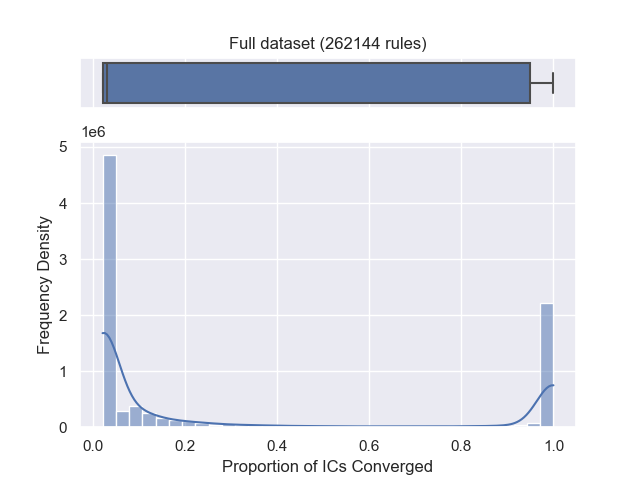
\includegraphics[width=.5\textwidth]{images/full-taxonomy.png}}\hfill
            \subfloat{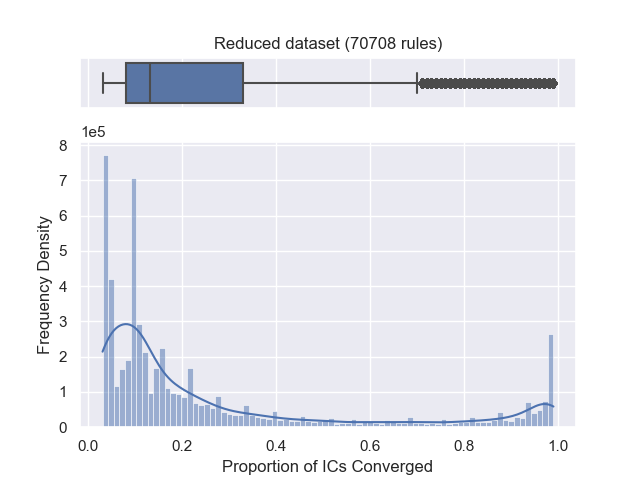
\includegraphics[width=.5\textwidth]{images/reduced-taxonomy.png}}\hfill
            \caption{Distributions of convergence of full and reduced set of life-like CAs}
\label{fig:taxonomy-dist}
\end{figure}

\subsection{Similarity Metrics}

It is useful to evaluate the manner in which the population converge towards solutions during evolution. Although we use the word convergence to describe this, it is important to note the difference between a CA converging to fixed point or periodic solution and a population converging towards an optimal transition function. To evaluate the convergence of a population, it is useful to have a notion of similarity between individuals. This allows us to quantify the speed of convergence and group individuals into families if they are converging towards different optima. For a binary string chromosome, the simple matching coefficient (SMC) between two individuals is an appropriate metric to quantify their relative similarity. 
\begin{definition}[Simple Matching Coefficient] Consider two binary strings $A$ and $B$. The frequency table enumerating the number of instances of each possible combination of bit settings is
\begin{center}
    \begin{tabular}{ c c c }
              & $A_i = 0$ & $A_i = 1$ \\ 
        $B_i = 0$ & $n_{0,0}$ & $n_{1,0}$ \\  
        $B_i = 1$ & $n_{0,1}$ & $n_{1, 1}$    
    \end{tabular}
\end{center}
The simple matching coefficient between two binary strings $A$ and $B$ of length $n$ is\\
\[
    SMC = \frac{n_{0, 0} + n_{1, 1}}{n_{0, 0} + n_{1, 1} + n_{0, 1} + n_{1, 0}}
\]
    
\end{definition}
Symmetrically, we consider the Simple Matching Distance, $\textnormal{SMD} = 1 - \textnormal{SMC}$, as a measure of diversity between individuals. This is appropriate as SMD fulfills all the formal criteria for a distance metric: non-negativity, symmetry, identity of indiscernibles, and the triangle inequality. If each bit is to be imagined as a gene, the SMD is the mean number of differing genes in the chromosome. It can be calculated in $O(n)$ time where $n$ is the chromosome length. Aside from being simple to understand and efficient to calculate, the SMD is preferable to other metrics as it counts mutual presence and mutual absence. Jaccard Distance $d_J$, on the other hand, only counts mutual presence. For two binary strings $A$ and $B$
\[
    d_J = \frac{n_{0, 1} + n_{1, 0}}{n_{0, 1} + n_{1, 0} + n_{1, 1}}
\]
Although this is useful in settings with many false negatives that ought to be ignored, our use case benefits from knowing when a gene is \textit{not present} in both chromosomes as much as knowing if it \textit{is present} in both. For this reason we use the Simple Matching Distance.

\section{Maze Generation}

We begin by evaluating the effectiveness of the maze generator at maximizing the two fitness metrics. These are the length of the solution path ($p$) and the number of dead ends ($d$). From spot checks on a few examples in the simulator, we find that these two metrics happen to have similar ranges (around 70-100). For this reason we begin by treating them with equal weighting during hyperparameter tuning.\\

\subsection{Hyperparameter Tuning}

We tune a bias parameter $\lambda$ to find which bias maximizes $\lambda \hat{p}_\lambda + (1-\lambda)\hat{d}_\lambda$ where $ \hat{p}_\lambda$ and $\hat{d}_\lambda$ are the optimal values discovered by the algorithm under a bias of $\lambda$.\\


\subsection{Roulette vs Truncation Selection}

As the population evolves, the variance in fitness decreases. This makes a roulette selection increasingly likely to pick suboptimal parents. Truncation selection, on the other hand, asserts that a selected candidate will never have a lower fitness than a candidate that has not been selected. However, this can increase the likelihood of premature convergence since genes within incrementally worse solutions that have potential to produce global optima are lost.\\

Since we are optimising for two metrics, we can take a linear combination of the objective values of $p$ and $d$ or we can rank each candidate separately by $p$ and $d$ then take a linear combination of the ranks. We call this objective and relative fitness respectively. As

\section{Life-Like CA}

When evaluating the effectiveness of evolutionary techniques at learning life-like CA rules, it is important to contextualise quantitative properties like convergence rate, fitness, and diversity. We begin by performing an exploratory statistical analysis to gather data on the life-like CA rule space. In conjunction with the analyses of Wolfram\cite{wolfram1986theory} and Eppstein\cite{eppstein2010growth}, this will shed light into the characteristics that make a rule easier or harder to predict.


\subsection{Special Case Evaluation}

We begin by attempting to learn for a few specific rules to test the efficacy of the learning process. Consider Conway's Life rule B3/S23. In binary this is '000100000001100000' and as an integer it is 16480. We use the following hyperparameters.
\begin{center}
    \begin{tabular}{ l c }
        Epochs & 30\\
        Population Size & 100\\
        Elitism Rate & 0.2\\
        Mutation Rate & 0.05\\
        Evaluation Steps & 10\\
        Minimum Step Size & 1\\
        Maximum Step Size & 10\\
    \end{tabular}
\end{center}
These have been obtained by looking at common parameters used in the literature and validating on a few examples to ensure quality of learning while minimizing computation time. A more rigorous hyperparameter tuning is covered in Subsection~\ref{sub:hyperparameter-tuning}. Moving forward, we assume this configuration unless otherwise stated. We begin by testing each CA on 20 initial conditions sampled from a distribution uniform on density. This early attempt at learning Life yields poor results.

\begin{figure}[!h]
\centering
            \subfloat[Scatter plot of chromosome values over learning period.]{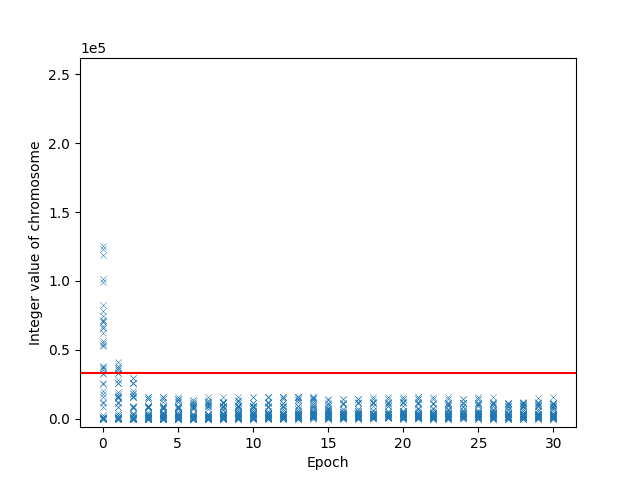
\includegraphics[width=.45\textwidth]{images/life_like_eval/nothing-big.png}}\hfill
            \subfloat[Empirical CDF distribution of chromosome values at epoch 30]{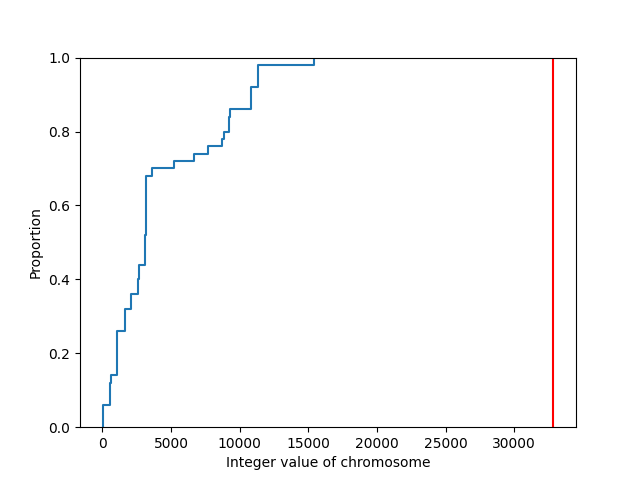
\includegraphics[width=.45\textwidth]{images/life_like_eval/nothing-cdf.png}}\hfill
            \caption{Learning Life using a genetic algorithm (20ICs). Red line indicates the goal.}
\label{fig:life-nothing}
\end{figure}

Figure~\ref{fig:life-nothing}(a) reveals that the algorithm converges to local optima below the global optimum. Figure~\ref{fig:life-nothing}(b) reveals that, at epoch 30, all individuals are below the goal with the majority lying around a value of 4000. To get a finer perspective on this, we run the experiment again with 100 initial conditions tested per CA.

\begin{figure}[!h]
\centering
            \subfloat[Scatter plot of chromosome values learnt with 100 ICs per CA]{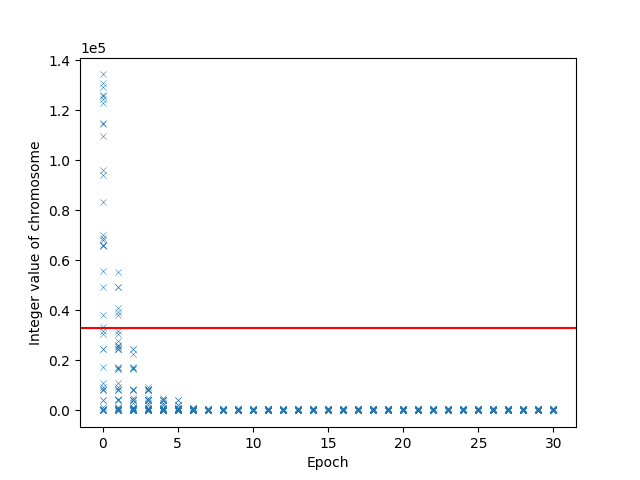
\includegraphics[width=.45\textwidth]{images/life_like_eval/nothing-big-100.png}}\hfill
            \subfloat[Same as figure (a) but zoomed into values $<1000$]{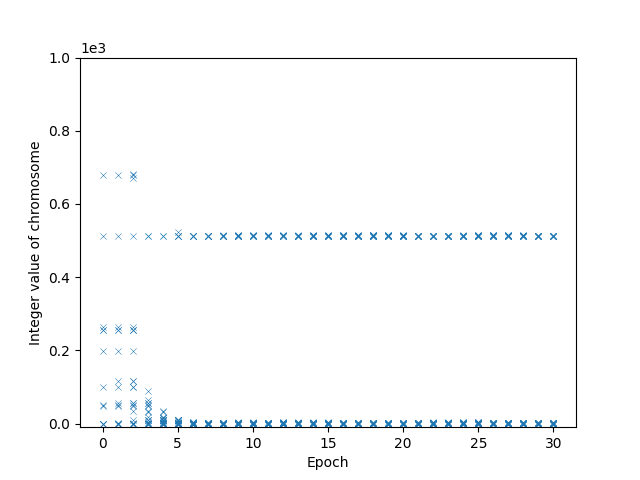
\includegraphics[width=.45\textwidth]{images/life_like_eval/nothing-small-100.png}}\hfill
            \caption{Learning Life using a genetic algorithm (100ICs)}
\label{fig:life-nothing}
\end{figure}

Here we see two clear locally optimal regions around 0 and 500 that all individuals have converged to. Running a value count on the final population reveals there are only 5 unique individuals $\{ 0, 1, 513, 514, 2 \}$ with frequencies $\{18, 14, 9, 5, 4 \}$ respectively. The top 4 correspond to the rules B/S, B/S8, B8/S, and B8/S8. Rules with empty birth sets mean that no dead cell can become alive so the system monotonically tends towards quiescence with all cells dead. The case is symmetrical with an empty surival set where the system tends towards the $\vec{1}$ quiescent state. Similarly, a birth or survival set of \{8\} is extremely unlikely to get triggered. These chromosomes with sparse birth and survival sends tend to promote inactivity in the predicted CA which grants them an edge over volatile chromosomes that quickly wipe themselves out.


\subsection{Hyperparameter Tuning}\label{sub:hyperparameter-tuning}

We begin by performing some crude hyperparameter testing on the genetic algorithm. Considering a random uniform stepsize, $\delta_k \sim \mathit{Uniform}(D_{max}, D_{min})$ we set $D_{min} = 1$ since we would like to give the algorithm a chance of learning on very small steps. To determine $D_{max}$, the algorithm is run on 100 goal rules and each the loss of each rule is calculated by simulating on 100 random initial conditions. By running the algorithm on populations of size 10 and 100 with $D_{max} \in \{1, 10, 100\}$ for 30 epochs, we find the highest proportion of experiments converging to the precise goal rule within 30 epochs when the population is of size 100 and $D_{max}$ is 10. With this configuration, 32\% of goals are precisely learnt. It is clear that population size makes a considerable difference on performance so for all future tests, we maintain a population size of 100.\\

\begin{figure}[!h]
\centering
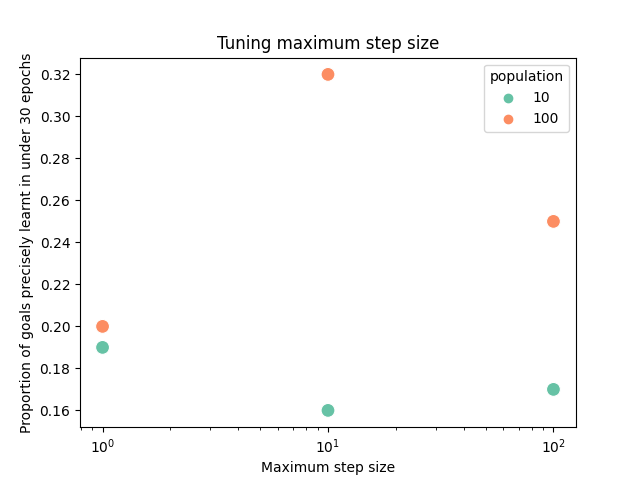
\includegraphics[width=0.7\textwidth]{images/tune-max-step.png}
\caption{Percentage of runs that converge within 30 epochs}
\label{fig:tune-max-step}
\end{figure}

In order to reduce training time when testing different hyperparameters, we reduce the size of the training set of initial conditions from 100 to 20. Although this somewhat compromises on the strength of the overall algorithm, it allows us to quickly compare multiple different configurations. One such choice is between loss functions. We consider the performance of the single resolution loss against the multiple resolution loss on a population of 100 over 30 epochs with 20 random initial conditions tested per individual.\\    


\subsection{Class-Wide Evaluation}


\section{Gray-Scott Models}